% !TeX root = ../main.tex
% Add the above to each chapter to make compiling the PDF easier in some editors.


\chapter{Introduction}\label{chapter:introduction}

An important topic in computer science is the study of the
\textit{functional correctness} of an algorithm.
It states whether an algorithm actually solves a problem
in the intended way.
This topic becomes especially interesting when it can be applied
to directly executable code and is machine checked.
Unfortunately with both desirable additions, the tasks becomes
significantly more complex.
In an abstract specification we may abstract away many consideration
an actual program has to be concerned with and are still
left with the obligatino to show non-trivial properties.
Furthermore for the concrete code we have to reason about specific low level
decisions such as memory allocation or
the eligibility of reusing variables.
In this thesis we provide a computer assisted proof for the functional
correctness of an imperative implementation of the B-Tree data-structure
and present how we dealt with the above mentioned issues.

In \autoref{chapter:introduction}, we introduce B-Trees and common variations
on them.
The variation that is most promising for our approach is chosen
to be implemented.
We first design a functional, abstract implementation.
Together with a proof of its functional correctness,
it is presented in \autoref{chapter:abs-set}.
On this level, functional correctness is equivalent with the
implementation of an abstract Set-interface,
that requires retrieval, insertion and deletion operations.
From there, an imperative implementation is derived in \autoref{chapter:imp-set}.
Its functional correctness is shown by proving that it refines the functional specification.
Thus the proof obligation for the imperative implementation
is reduced to a proof of equivalence between the output of the
functional and the imperative implementation.
This gives freedom for low-key optimizations with regard to a naive translation.
Finally, we present learned lessons, compare the results with related work and suggest potential future
research in \autoref{chapter:conclusion}

% TODO related work?
% mfp/fielding: not mechanized, different approaches
% Ernst: more automation, but actually similar approach to ours (except for used structure)
% Malecha: less automation, similar structure

We realize that the verification of B-Trees or the related B$^+$-Trees
is a hard problem.
The first rigorous approaches at it to our knowledge are the works by Fielding \parencite{Fielding80}
and Sexton \parencite{DBLP:journals/entcs/SextonT08}.
Both were not machine checked but shed light on both techniques applied in this work.
Fielding approaches the verification by iterative refinement of an abstracted
specification which we emply in \autoref{chapter:abs-set}.
Sexton uses the sophisticated tool of separation logic to reason directly 
on imperative specification, in a similar manner to our specification in \autoref{chapter:imp-set}.
\parencite{DBLP:journals/sosym/ErnstSR15} also directly verify an imperative
implementatione by combining interactive theorem proving 
with shape analysis.
The main recursive procedures interactively are interactively verified in KIV.
Data structure properties such as circle-freeness are then proven by shape-analysis.
Another direct proof on an imperative specification 
can be found in \parencite{DBLP:conf/popl/MalechaMSW10}, with the YNOT
extension to the interactive theroem prover Coq.


\section{The Isabelle Proof Assistant}

Isabelle/HOL is an interactive theorem prover that allows
to reason, among other things, in Higher Order Logic.\parencite{DBLP:books/sp/NipkowPW02}
It is built ML, which influences the syntax of functional
programs written in it.
Isabelle code is portioned in so called theories,
roughly being equal to a module in common languages.
A theory consists of the specification of datatypes,
typed functional programs and theorems with proofs.

\subsection{Notation and proofs in Isabelle}

Functions, predicates and the like are all expressed in
a functional manner.
\textbf{definition} denotes classical definitions and \textbf{fun}
is used for recursive definitions.
The latter is only a valid definition if it incorporates an automatic proof of termination.
Usually this proof is done automatically however.
If a function evaluation does not terminate for all inputs
it is denoted with \textbf{partial\_fun}.
The term \textbf{abbreviation} refers to a simple shorthand for more complex expressions,
similar to a macro.

Lemmas, theorems and the like can be expressed in a similar manner
as they would be written in mathematical textbook.
They begin with i.e. \textbf{lemma}, followed by an
expression or predicate and a proof that it holds.
Wherever possible and readable, we will try to reflect the actual
syntax of the Isabelle system.
To prove a theorem correct, the system basically provides two different
proof styles.

One option is to write structured proofs in the isar language.
The user outlines a proof with intermediate goals
and tells the system which proof methods to apply to
resolve each step.
This method is usually preferred as it is more readable and usually
faster on the system side.
All complex proofs in \autoref{chapter:abs-set} are hence written in this style.

In the apply style, the user tells the system which proof method
to apply to modify the current goal.
This is practical if the number of assumptions
is high or the goal is large and writing the full terms
out would be impractical.
Since this is the case for the proofs of the imperative programs,
almost all proofs in \autoref{chapter:imp-set} are written in this style.
In this work we will not present the proofs as written in the actual
proof files but rather outline the structure of the proofs.

The system provides a number of proof methods,
based on different manipulation tools
such as logical reasoning or simplification.
When mentioning \textit{automatic} proofs, we mean a proof that
comprises very few ($\le 5$) apply style
invocations of proof methods is meant.
A method that commonly allows for such proofs is the \textit{auto} method,
a combination of logical reasoning and repeated simplification,
but also allowing automatic case distinctions and destructive rule application.

\subsection{Examples and basics of the Isabelle language}

Datatypes may be defined recursively.
The following shows as an example the internal definition of the list datatype.\footnote{
    The actual definition is worded slightly different but this is of no importance here.
}

\begin{lstlisting}[mathescape=true, language=Isabelle,label=lst:list-def]
datatype 'a list = [] | 'a # 'a list
\end{lstlisting}

In natural language this means that either a list is the empty list,
or it is an element prepended on another list.
As usual in ML like languages, we may deconstruct an argument to a function
by pattern matching to this construction.
In addition, the type $'t$ of any expression $e$ can be
made explicit by writing \textit{e :: 't}.
Functions that take values of type $'a$ and return values of type $'b$ 
have type \textit{'a $\Rightarrow$ 'b}.
The Isabelle internal list catenation function serves as
an example for a function definition with explicit type.

\begin{lstlisting}[mathescape=true, language=Isabelle,label=lst:append-def]
fun (@) :: 'a list $\Rightarrow$ 'a list $\Rightarrow$ 'a list where
    [] @ ys = ys |
    (x#xs) @ ys = x # (xs @ ys)
\end{lstlisting}

% TODO include?
% locales
% set specification
It is possible to specify functions, predicates
and theorems with respect to some abstracted function
of which only certain properties are known,
resulting in so-called \textbf{locales}.

Further details on notation, proof techniques and more in Isabelle/HOL
may be found in \parencite{DBLP:books/sp/NipkowPW02}.


\section{The B-Tree Data Structure}

B-Trees were first proposed by Bayer et al. in \parencite{DBLP:journals/acta/BayerM72},
as a data-structure to efficiently store and retrieve indices stored on storage devices
with slow memory access.
They are $n$-ary balanced search trees, where each
node contains many indices.
The number of subtrees and indices in each node is defined by the \textit{order} $k$ of the tree.
% TODO reorder with definitions
B-Trees are a generalization of 234-Trees and a specialization of (a,b)-Trees
A common variation is the B$^+$-Tree, where the inner nodes
only contain orientation yielding separators
but all elements are eventually stored in the leaves. 
\parencite{DBLP:journals/csur/Comer79}
Note that usually B-Trees are supposed to implement a map-like
structure, where each element is an index together with a pointer
or some arbitrary additional data.
However for the sake of keeping the implementation and proofs simple,
and first showing the validity of the approach in this case,
we say that B-Trees store some linearly ordered values
that themselves form the elements of an concretized set.

\subsection{Definitions}
\label{sec:data_structure_defs}

Every node contains a list of \textit{keys} (also \textit{separators}, index elements), and \textit{subtrees},
that refer to further B-Trees.
The separators and subtrees may be considered considered interleaved within a node,
such that we can speak of a subtree left of a separator and a subtree right of a separator,
where for a separator at index $i$ we mean the subtree in the respective
subtree list at index $i$ and $i+1$ respectively.
Note that this already implies that the list of subtrees is one
longer than the list of separators - we refer to the last subtree
as the \textit{last} or \textit{dangling} subtree.
In \parencite{DBLP:journals/acta/BayerM72},
a B-Tree with above structure must fulfill the three properties
\textit{balancedness}, \textit{order} and \textit{sortedness}.

\paragraph{Balancedness} \textit{Balancedness} requires
that each path from the root to any leaf has the same length $h$.
In other words, the height of all trees in one level of the tree must be equal.
This is possible to accomplish due to the flexible amount of subtrees
in each node.

\paragraph{Sortedness} Further the indices must be \textit{sorted} within the tree which means that all indices stored
in the subtree left of a separator are smaller than the value of the separator
and all indices on the right are greater.
Further all indices within a node should maintain a sorted order.

\paragraph{Order} In general terms, the property of \textit{order} ensures a certain minimum and maximum
number of subtrees for each node.
However, as pointed out in \parencite{DBLP:books/daglib/0095349_mod},
the property is defined differently in the literature.
For the purpose of this work, the original definition by Bayer et al. was chosen as most suitable.
A B-Tree is of order $k$, if each internal node has at least $k+1$
subtrees and at most $2k+1$.
The alternative of defining the nodes to have between $\lceil \frac{k}{2} \rceil$
and $k$ children (as proposed in \parencite{DBLP:books/lib/Knuth98a}),
involves cumbersome \textit{real} arithmetic that unnecessarily complicates
mechanized proofs.
Sticking to the original definition is further supported by the fact that nodes are supposed
to fill memory pages which are usually of even size (usually some power of 2).
An even number of separators and trees plus one dangling last right tree maximizes
the usage of such a page.

The same ambiguity exists for the term \textit{Leaf} which we will define consistently with Knuth's definition \parencite{DBLP:books/lib/Knuth98a}
to be an empty node, carrying no information,
rather than a node without children.
This is close to the usual approach in functional programming,
and will yield elegant recursive equations for our B-Tree operations.
The lowest level of nodes hence contains a list of separators and
list of pointers to leaves.

Note that the B-Tree definition is only meaningful for positive $k$.
For the case that $k$ is equal to 0,
all elements of the tree would have exactly one subtree
and no internal elements.
For the root node this even leads to a contradictory state:
It is required to contain at least 1 element.
However as it should not have more than $2k = 0$ elements,
this constraint cannot be satisfied.
Requiring positive $k$ is consistent with the definitions
in the literature consulted \parencite{DBLP:journals/acta/BayerM72,DBLP:journals/csur/Comer79,DBLP:books/daglib/0023376}

% insert image of valid B-Tree
A simple example B-Tree may be seen in \autoref{fig:btree-basic-nopair}.
Nodes and Leafs are represented as circles, were the former points to the
subtree that a node represents and the latter is left empty.

\begin{figure}
    \centering
    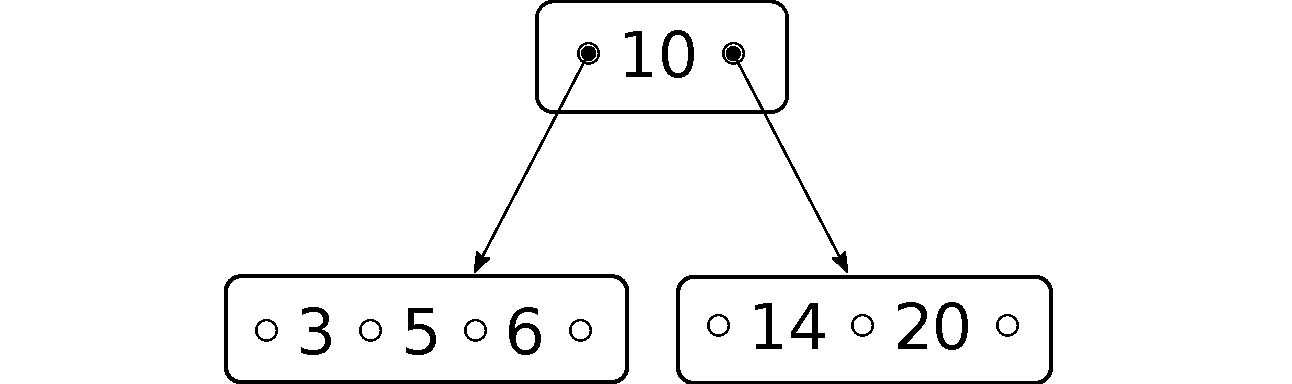
\includegraphics[width=0.5\linewidth]{figures/btree-basic-nopair.pdf}
    \caption{A small balanced B-Tree of order $2$ and
    height $2$ containing $3$ nodes and $6$ elements.
    Circles represent nodes, where empty circles are leafs and filled circles
    point to the corresponding subtree.}
    \label{fig:btree-basic-nopair}
\end{figure}

\subsection{B-Tree operations}

The B-Tree is a dynamic data-structure and provides
a number of operations to inspect or modify the stored data.
Generally the operations are defined recursively on the nodes.
The correct subtree may be found by inspecting the separators stored
in the currently visited node.
If the value that is being searched for is in the range of two
adjacent separators, the tree in between is the correct for recursion. 
The obvious corner cases are if the value is less than the
minimal element or greater than the maximum element stored.
In that case we recurse in either the first or the last subtree.
The exact manner of inspection should in practice of course
be efficient and will hence be kept abstract until \autoref{chapter:imp-set}.

\paragraph{Retrieval}\label{par:intro-isin}
Since the whole tree is sorted,
checking whether certain elements are contained in the tree
is simply conducted by recursing into the correct node
in each level.
Either the element is found directly or found at a lower level.
If we reach a leaf node we know that the element is not contained in the tree.
There is little variation on this algorithm so there is no need for comparison.

% TODO move abstract discussion to introduction
%-------------------------------------------------
\paragraph{Insertion}\label{par:intro-ins}
There is also much consensus in the literature on how to conduct insertion into a B-Tree.
\parencite{DBLP:journals/csur/Comer79}
%TODO citations
%TODO relationship to other implementations (are there more?)
Generally, an element is inserted into the nodes on the lowest level.
In case that there is enough space left, the element is simply placed at the correct
position in the list of separators.
However if the node has more than $2k$ elements after this insertion,
we need to split it and, passing the median to the parent node,
recurse back upwards.
We will see in \autoref{sec:abs-ins} how this can be
elegantly expressed in a functional specification.
%-------------------------------------------------

% TODO delete
% TODO move abstract discussion to introduction
%-------------------------------------------------
\paragraph{Deletion}\label{par:intro-del}
On deletion, elements are removed from the leaves only.
If the element to be deleted resides in an inner node,
it is replaced by the maximal lesser or minimal greater
element in the tree, which always resides in a leaf
to the left or right of the element to be removed.

After deletion, the nodes may need rebalancing in order
to ensure the order property.
A node having less than $k$ elements is called to have \textit{underflow}.
However, opposing to the insertion function,
the exact procedure to handle underflow varies strongly in the literature.
Since only one element is removed from the node,
the most intuitive remedy to underflow is to \textit{steal} or \textit{borrow} it
from the left or right sibling.\parencite{DBLP:books/daglib/0023376}
If the left or right sibling has more than $k$ elements,
one of the neighboring elements may be moved out for increasing
the size of the current node.
Only in case that both siblings have left only $k$ elements,
a kind of reversal of the insertion split is conducted:
One of the siblings and the node itself are merged to form
a new, bigger node of valid order.

Following the description of \parencite{DBLP:journals/acta/BayerM72},
as done by \parencite{Fielding80},
the two cases can be treated identically.
If a node has less than $k$ elements,
merge it with one of its siblings.
If the resulting catenated node has an overflow again,
it will be split in half, just as with insertion related overflows.
According to \parencite{DBLP:journals/csur/Comer79} this may even be
more efficient than stealing single single keys from siblings.
First of, the resulting node is less likely to underflow again.
If it had stolen only one item, the probability for another underflow at the next
deletion is higher than if several elements are copied over.
Further, the node to merge with has to be read from memory anyways.
The cost of moving around up to $k$ elements that already reside in memory
is hence negligible compared to the cost of another underflow.

%-------------------------------------------------

\subsection{Properties}

B-Trees are assumed to be stored on external memory,
such that each node roughly matches a page in main memory.
Due to the potentially large branching factor and the balancing,
the number of required memory accesses for retrieving data stays small even for
large amounts of data stored.
This is due to the fact that the overall number of memory accesses is bounded by the depth
of the tree, which again is logarithmic in the number of indices -
where the base of the logarithm is closely proportional to the order $k$ of the tree.

Further, by design, the storage usage of B-Trees is at a minimum close to $50\%$,
where the average usage is usually higher. \parencite{DBLP:journals/acta/BayerM72}
This is due to the fact that every node reserves the storage of $2k$ keys and separators
but by definition always contains at least $k$ elements.

B-Trees build the foundation to most modern relational database implementations.
The above mentioned properties are key to the widespread popularity of B-Trees and are
hence preserved in the given implementation.
% TODO more
